\chapter{低成本无人机定位系统模型与定位理论基础}
\label{ch:fundamentals}

\section{系统任务场景与总体架构}
\label{sec:2_1}

\subsection{非合作终端定位任务描述}
\label{subsec:2_1_1}

复杂环境下手机直连卫星场景中的地面非合作终端快速发现与准确定位，是无线电安全监管中的重要任务。本文所称目标主要指具备卫星直连能力、但不向外部监测系统提供可信位置和同步辅助的地面终端，例如直接接入低轨卫星网络的手机。随着 3GPP NTN和 Direct-to-Cell 技术发展，普通手机直接接入低轨卫星网络的可行性和工程形态已得到系统研究与实测验证\cite{Lin2021NTN,He2024DirectSmartphone,GarciaCabeza2025DirectToCell}。与传统蜂窝网络中的常规定位任务相比，该类终端排查主要面临三方面困难：其一，目标通常不主动提供同步信息、位置信息或协议辅助信息，因此本质上属于非合作式无源定位问题\cite{Torrieri1984PassiveLocation}；其二，目标多位于建筑密集区域或复杂城市边缘地带，遮挡、反射、绕射与散射普遍存在，理想视距条件难以长期成立；其三，目标可能呈现临时出现、短时工作、动态移动甚至多目标并发辐射等复杂形态，这对系统的机动响应能力、连续跟踪能力和抗虚警能力提出了更高要求\cite{Wymeersch2009CooperativeLocalization}。

从任务目标上看，本文所研究的非合作终端排查并不局限于简单的信号检测，而是要求在复杂城市环境中实现对目标空间位置的有效估计。若将离散时刻 $k$ 场景中的目标集合表示为
\begin{equation}
\mathcal{X}_{k}
=
\left\{
\mathbf{x}_{k,i}
\right\}_{i=1}^{N_k},
\quad
\mathbf{x}_{k,i}
=
\left[
x_{k,i},\,
y_{k,i},\,
\dot{x}_{k,i},\,
\dot{y}_{k,i}
\right]^T,
\label{eq:2_1_target_state}
\end{equation}
其中，$N_k$ 表示时刻 $k$ 场景中的目标数量，$\mathbf{x}_{k,i}$ 表示第 $i$ 个目标的状态向量，$x_{k,i}$ 与 $y_{k,i}$ 表示其二维位置坐标，$\dot{x}_{k,i}$ 与 $\dot{y}_{k,i}$ 表示其速度分量，则非合作终端排查任务的本质可理解为：在目标数量未知、状态未知、传播条件复杂且观测受扰动影响的条件下，依托外部观测手段对 $\mathcal{X}_k$ 进行估计，并进一步实现对目标空间分布与运动状态的判定。

为了对上述问题进行统一描述，可将无人机平台对目标的定位过程抽象为多目标观测集合模型
\begin{equation}
\mathcal{Z}_{k}
=
\left\{
\mathbf{z}_{k,j}
\right\}_{j=1}^{M_k},
\quad
\mathbf{z}_{k,j}
=
h(\mathbf{x}_{k,\pi(j)})+\mathbf{v}_{k,j},
\label{eq:2_2_observation_model}
\end{equation}
其中，$\mathcal{Z}_k$ 表示第 $k$ 时刻接收到的观测集合，$M_k$ 表示对应时刻可获得的观测数量，$\mathbf{z}_{k,j}$ 表示第 $j$ 个观测向量，$\pi(j)$ 表示该观测所对应的目标索引，$h(\cdot)$ 表示由目标状态到观测空间的非线性映射关系，$\mathbf{v}_{k,j}$ 表示观测噪声及环境扰动项。式~\eqref{eq:2_2_observation_model} 表明，定位系统的输出精度不仅取决于目标状态本身，还与传播环境、观测方式以及噪声水平密切相关。对于复杂城市环境中的非合作终端排查而言，映射函数 $h(\cdot)$ 往往不再满足理想自由空间条件下的简单形式，而是受到多径传播、非视距遮挡和局部信号衰落的共同影响\cite{Torrieri1984PassiveLocation,Wymeersch2009CooperativeLocalization}。

\subsection{无人机定位系统总体架构}
\label{subsec:2_1_2}

本文所研究的低成本无人机定位系统总体架构如图~\ref{fig:ch2_uav_localization_scenario} 所示。该系统由低轨卫星、地面非合作终端、复杂城市传播环境、无人机机动观测平台以及后端定位处理链路共同构成，其中地面非合作终端对应前文所述的手机直连卫星目标。

\begin{figure}[htbp]
    \centering
    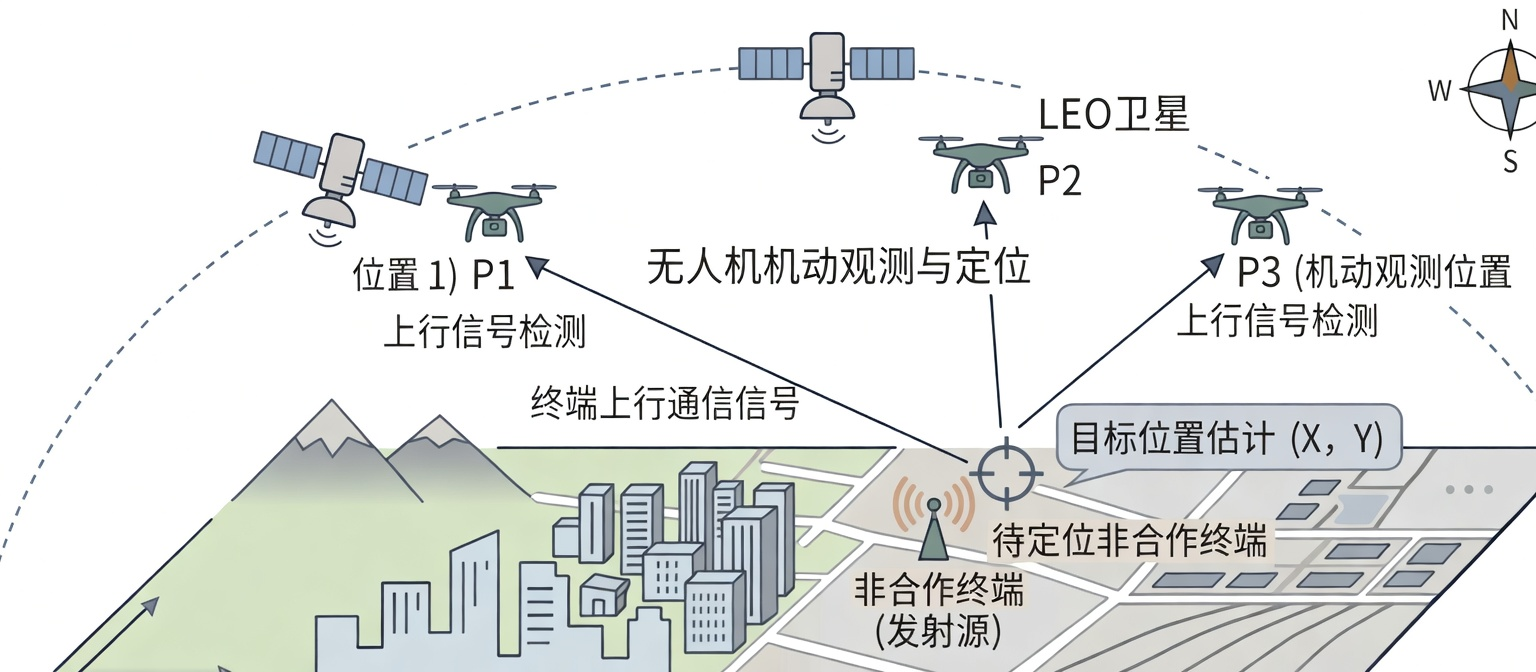
\includegraphics[width=0.82\textwidth]{figures/ch2/1_无人机机动观测下非法终端定位场景示意图.jpg}
    \caption{无人机机动观测下的非合作终端定位场景}
    \label{fig:ch2_uav_localization_scenario}
\end{figure}

从场景关系上看，低轨卫星与地面终端之间构成星地业务链路，地面终端则是无人机定位系统所关注的目标对象。目标相关信号在复杂城市环境中传播时，会受到建筑遮挡、反射、绕射和散射等因素影响，从而形成非理想传播条件。无人机通过多个机动观测位置对目标区域进行巡检接收，逐步形成对目标的空间观测几何与时序观测链路。

从信息流角度看，无人机平台在不同空间位置接收到目标相关信号后，系统进一步提取接收信号强度、到达方向、时间特征、轨迹递推信息以及后续方法中涉及的特征表示等观测信息。这些观测量或特征并不直接等同于最终位置，而是作为定位解算的输入，经由相应模型或学习算法进一步映射为目标位置估计结果。也就是说，整个定位过程本质上是一个从空间信号观测到目标状态参数的映射过程。第三章将利用这类机动观测信息构建面向单目标连续定位的自适应融合框架，第四章则进一步将空间采样结果组织为无线电地图，用于多目标并发定位中的信号成像与判别。

为了对图~\ref{fig:ch2_uav_localization_scenario} 所示过程进行统一描述，可将无人机定位系统抽象为离散时间状态空间模型
\begin{equation}
\mathbf{x}_{k}
=
f(\mathbf{x}_{k-1},\mathbf{u}_{k-1})+\mathbf{w}_{k-1},
\label{eq:2_3_state_equation}
\end{equation}
\begin{equation}
\mathbf{z}_{k}
=
h(\mathbf{x}_{k})+\mathbf{v}_{k},
\label{eq:2_4_measurement_equation}
\end{equation}
其中，$\mathbf{u}_{k-1}$ 表示上一时刻对系统状态演化有影响的输入量，$f(\cdot)$ 为状态转移函数，$\mathbf{w}_{k-1}$ 为过程噪声；$\mathbf{z}_k$ 表示第 $k$ 时刻无人机获得的观测向量，$h(\cdot)$ 为观测映射函数，$\mathbf{v}_k$ 为观测噪声。式~\eqref{eq:2_3_state_equation}--式~\eqref{eq:2_4_measurement_equation} 给出了后续章节讨论定位问题的统一数学框架：目标状态随时间演化，而观测则由目标状态经过复杂传播与测量过程映射得到。在单目标连续定位场景下，$\mathbf{x}_k$ 可表示单个目标终端的位置或运动状态；在多目标场景下，该模型可进一步扩展为上一小节给出的目标集合状态描述。总体而言，本文所研究的低成本无人机定位系统，本质上是一个以无人机机动观测为核心、以复杂环境下信号感知为基础、以目标位置估计为输出的动态定位系统，后续研究需要在此基础上进一步结合复杂城市环境下的传播机理与观测误差来源展开分析。


\section{低轨卫星信号模型}
\label{sec:2_2}

\subsection{多径效应、时延扩展与信号衰落机制}
\label{subsec:2_2_1}

在复杂城市环境下，低轨卫星终端相关信号从发射端传播至无人机接收端的过程中，通常不会仅沿单一直达路径传播，而是会受到建筑物立面、街道边缘、玻璃幕墙以及地表散射体的共同影响，形成由直达径、反射径、绕射径和散射径叠加构成的复合传播过程。对于非合作低轨卫星终端排查任务而言，这种传播条件的复杂化将直接改变接收端所观测到的信号结构，使理想环境下基于简单几何关系建立的定位模型难以长期成立。因此，在建立后续定位方法之前，有必要先从传播层面对多径效应、时延扩展以及信号衰落机制进行统一分析\cite{TR38901,Guvenc2009TOASurvey}。

从信号模型角度看，若接收端共接收到 $L$ 条有效传播路径，则复基带接收信号可表示为
\begin{equation}
r(t)
=
\sum_{l=1}^{L}
\alpha_l
\,s(t-\tau_l)\,
e^{-j2\pi f_c\tau_l}
+
n(t),
\label{eq:2_5_multipath_signal}
\end{equation}
其中，$s(t)$ 为发射信号，$\alpha_l$ 和 $\tau_l$ 分别表示第 $l$ 条路径的复衰落系数和传播时延，$f_c$ 为载波频率，$n(t)$ 为加性噪声。式~\eqref{eq:2_5_multipath_signal} 表明，接收端实际观测到的信号是多条传播路径在幅度、相位和时延上的叠加结果，而非理想自由空间条件下的单一路径传输结果。

在复杂城市环境中，当无人机与目标终端之间存在视距链路时，接收信号中往往同时包含直达径与若干条反射路径；而当建筑物遮挡导致直达路径被阻断时，系统只能接收到经墙面反射、边缘绕射或局部散射后到达的非视距分量。此时，接收端观测信号不仅信噪比下降，而且其主导路径的几何意义也会发生偏移。例如，在方向估计问题中，最强到达路径的方向可能不再指向真实目标；在功率测距问题中，接收功率也会偏离理想路径损耗模型所对应的单调衰减关系。由此可见，多径效应带来的影响并不局限于噪声增强，而是会从根本上改变观测量与真实位置之间的映射关系。

为了更紧凑地描述多径传播结构，通常可引入信道冲激响应表示。对于时变城市传播环境，等效信道可写为
\begin{equation}
h(t,\tau)
=
\sum_{l=1}^{L}
\alpha_l(t)
e^{-j\phi_l(t)}
\delta\big(\tau-\tau_l(t)\big),
\label{eq:2_6_time_varying_cir}
\end{equation}
其中，$\alpha_l(t)$、$\phi_l(t)$ 和 $\tau_l(t)$ 分别表示第 $l$ 条路径在时刻 $t$ 的幅度、相位和传播时延。式~\eqref{eq:2_6_time_varying_cir} 说明，复杂城市环境中的信道本质上是由若干条随时间变化的多径分量共同构成的。对于无人机平台而言，由于平台自身处于运动状态，接收端的相对观测几何会随航迹不断变化，因此多径结构不仅受环境决定，也会随无人机位置变化而动态演化。

在多径环境下，不同路径具有不同到达时延，从而导致接收信号能量在时域上被拉宽。为了度量这一离散程度，通常定义平均时延和均方根时延扩展。设第 $l$ 条路径的平均功率为 $P_l$，则平均时延可表示为
\begin{equation}
\bar{\tau}
=
\frac{\sum_{l} P_l \tau_l}{\sum_{l} P_l},
\label{eq:2_7_mean_delay}
\end{equation}
对应的均方根时延扩展为
\begin{equation}
\sigma_{\tau}
=
\sqrt{
\frac{\sum_{l} P_l(\tau_l-\bar{\tau})^2}{\sum_{l} P_l}
},
\label{eq:2_8_rms_delay_spread}
\end{equation}
其中，$\sigma_{\tau}$ 越大，表明信号能量在时域上的分散程度越高，接收端越难稳定区分主导路径与附加路径。对于定位任务而言，时延扩展的增大通常意味着传播环境更复杂，路径重叠更严重，观测结果更容易受到多径干扰。

需要指出的是，均方根时延扩展不仅是传统无线传播分析中的重要参数，在本文后续方法中也具有直接作用。在第三章中，$\sigma_{\tau}$ 将被作为表征传播复杂度的重要物理感知特征，参与融合权重预测模型的特征构造；在第四章中，由多径引起的时域离散和空间叠加效应，又会进一步表现为空间热力图中的局部高亮扩散、纹理模糊和伪热点增强。因此，从论文整体逻辑来看，时延扩展不仅是一个信道统计量，也是连接传播机理与后续定位学习方法的重要桥梁。

除时域离散外，多径传播还会引起显著的功率衰落与信号起伏。若仅从大尺度传播角度考察，接收功率常采用对数距离模型描述：
\begin{equation}
P_r(d)
=
P_t
-
PL(d_0)
-
10n\log_{10}\frac{d}{d_0}
+
X_{\sigma},
\label{eq:2_9_log_distance_model}
\end{equation}
其中，$P_t$ 为发射功率，$PL(d_0)$ 为参考距离 $d_0$ 处的路径损耗，$n$ 为路径损耗指数，$X_{\sigma}$ 为阴影衰落项。式~\eqref{eq:2_9_log_distance_model} 表明，即使在相同几何距离条件下，接收功率也会因环境遮挡、建筑分布和局部传播条件差异而出现明显波动。在城市峡谷环境中，这种波动通常表现得更为剧烈，从而使 RSSI 与传播距离之间的对应关系明显弱化\cite{TR38901}。


\subsection{外部观测信号模型}
\label{subsec:2_2_2}

本文关注的是无人机平台对地面非合作目标的外部观测，而不是对具体卫星通信协议的完整解析。考虑到不同手机直连卫星系统在空口体制、频段配置和调度方式上可能存在差异，本文从定位建模角度采用等效接收信号模型描述目标信号在复杂环境中的传播过程。设目标发射的等效基带信号为 \(s_u(t)\)，则第 \(i\) 个无人机观测位置接收到的复基带信号可表示为
\begin{equation}
r_i(t)
=
\sum_{l=1}^{L}
\alpha_l(t)
s_u\big(t-\tau_l(t)\big)
e^{j2\pi \nu_l(t)t}
+
n_i(t),
\label{eq:2_10_external_received_signal}
\end{equation}
其中，\(L\) 表示有效传播路径数，\(\alpha_l(t)\)、\(\tau_l(t)\) 和 \(\nu_l(t)\) 分别表示第 \(l\) 条路径的复衰落系数、传播时延和多普勒频移，\(n_i(t)\) 表示第 \(i\) 个观测位置的接收噪声。式~\eqref{eq:2_10_external_received_signal} 表明，无人机接收到的目标信号同时包含发射波形、复杂城市多径传播、平台相对运动和接收噪声等因素。对于后续定位而言，系统并不要求完全恢复通信协议，而是从该接收信号中提取 RSSI、AoA、TOA/TDOA 相关量以及 RMS 时延扩展等可用于定位和状态感知的观测特征。

近年来，Direct-to-Cell 以及 3GPP NTN 相关研究表明，普通手机直接接入低轨卫星网络正在成为可部署的通信形态\cite{Lin2021NTN,He2024DirectSmartphone,GarciaCabeza2025DirectToCell}；同时，LEO 定位和直接到终端通信定位一体化研究也说明，卫星网络可为终端定位提供新的几何与信号条件\cite{Dureppagari2025LEOPositioning,DeGaudenzi2026D2DPartI,DeGaudenzi2026D2DPartII}。但在本文的监管排查场景中，目标不主动参与定位，不提供可信 GNSS 坐标和同步辅助，因此不能简单假设系统能够获得网络侧完整定位量。基于这一约束，后续章节主要研究如何利用无人机外部观测形成稳健的位置估计与自适应融合定位。

\section{经典定位方法}
\label{sec:2_3}

在前文中，本文已经对非合作低轨卫星终端排查任务场景、系统总体架构以及低轨卫星信号模型进行了分析。可以看到，信号在从地面发送至无人机的过程中，会受到多径叠加、阴影衰落和非视距遮挡的共同影响，这些因素直接决定了接收端所获取观测量的质量。为了建立后续定位方法的基础，本节首先对 RSSI、AOA、TOA、TDOA 和 PDR 等经典定位方法的基本模型总结\cite{Torrieri1984PassiveLocation,Wymeersch2009CooperativeLocalization}。

\subsection{RSSI 定位}
\label{subsec:2_3_1}

接收信号强度指示（Received Signal Strength Indicator, RSSI）定位是一类基于信号功率衰减特性的经典定位方法，其基本思想是利用接收端测得的信号强度与传播距离之间的统计关系，反推出目标与观测平台之间的相对距离，再结合多个观测位置的几何关系实现目标位置估计。由于 RSSI 可直接由接收信号获取，对额外同步机制和复杂阵列结构的依赖较弱，因此该方法在低成本定位场景中具有实现简单、部署方便和计算开销较低等优点。

在理想自由空间条件下，信号功率随传播距离增大而逐渐衰减，其基本规律可由路径损耗模型描述。若采用对数距离路径损耗模型，则距离 $d$ 处的接收功率可写为
\begin{equation}
P_r(d)
=
P_t
-
PL(d_0)
-
10n\log_{10}\frac{d}{d_0}
+
X_{\sigma},
\label{eq:2_15_rssi_pathloss_model}
\end{equation}
其中，$P_t$ 为发射功率，$PL(d_0)$ 为参考距离 $d_0$ 处的路径损耗，$n$ 为路径损耗指数，$X_{\sigma}$ 为阴影衰落项。若暂不考虑随机扰动项，则可以根据接收功率反推出目标到观测点之间的距离估计值
\begin{equation}
\hat d
=
d_0
\cdot
10^{\frac{P_t-PL(d_0)-P_r(d)}{10n}}.
\label{eq:2_16_rssi_distance_estimation}
\end{equation}
式~\eqref{eq:2_16_rssi_distance_estimation} 给出了 RSSI 测距的基本形式。对于单个观测点而言，$\hat d$ 对应的是一个以观测点为圆心、以估计距离为半径的等距圆；当无人机平台在多个空间位置获得 RSSI 观测时，即可形成多个距离约束，并通过几何交会估计目标位置。若第 $i$ 个观测位置坐标为 $(x_i,y_i)$，目标位置为 $(x,y)$，则对应的几何关系可写为
\begin{equation}
\sqrt{(x-x_i)^2+(y-y_i)^2}
=
\hat d_i,
\qquad i=1,2,\dots,M,
\label{eq:2_17_rssi_geometry_constraint}
\end{equation}
其中，$M$ 为有效观测位置数，$\hat d_i$ 为第 $i$ 个观测位置对应的 RSSI 测距结果。当 $M\geq 3$ 时，理论上可通过最小二乘等方式求解目标位置。


\subsection{AOA 定位}
\label{subsec:2_3_2}

到达角（Angle of Arrival, AOA）定位是一类基于信号空间传播方向的经典定位方法。其基本原理是利用具有方向性感知能力的接收天线阵列，通过测量入射信号在阵列上的相位差或功率分布，估计信号相对于观测平台的到达方位角，并根据测量出的方位线与多个观测位置的几何关系实现对目标的定位。

设目标在地面二维平面上的坐标为 $\mathbf{x} = [x, y]^T$，第 $i$ 次观测时无人机的空间位置坐标为 $(x_i, y_i)$，则其观测到的目标方位角 $\theta_i$ 与目标位置之间的几何关系为
\begin{equation}
\theta_i
=
\mathrm{atan2}(y-y_i,\,x-x_i)
+
\epsilon_{\theta,i},
\label{eq:2_18_aoa_observation_model}
\end{equation}
其中，$\epsilon_{\theta,i}$ 为角度测量噪声。式~\eqref{eq:2_18_aoa_observation_model} 表明，一次 AOA 观测可以在空间中确定一条以观测点为起点、指向目标方向的方位射线。当无人机在多个不同位置开展机动观测时，可以形成多条方位射线的交会，从而确定目标位置。

图~\ref{fig:ch2_aoa_localization} 展示了 AOA 定位的几何原理。该图突出了无人机在不同航迹点获取方位射线，并由射线交点反推目标位置的过程。

\begin{figure}[htbp]
    \centering
    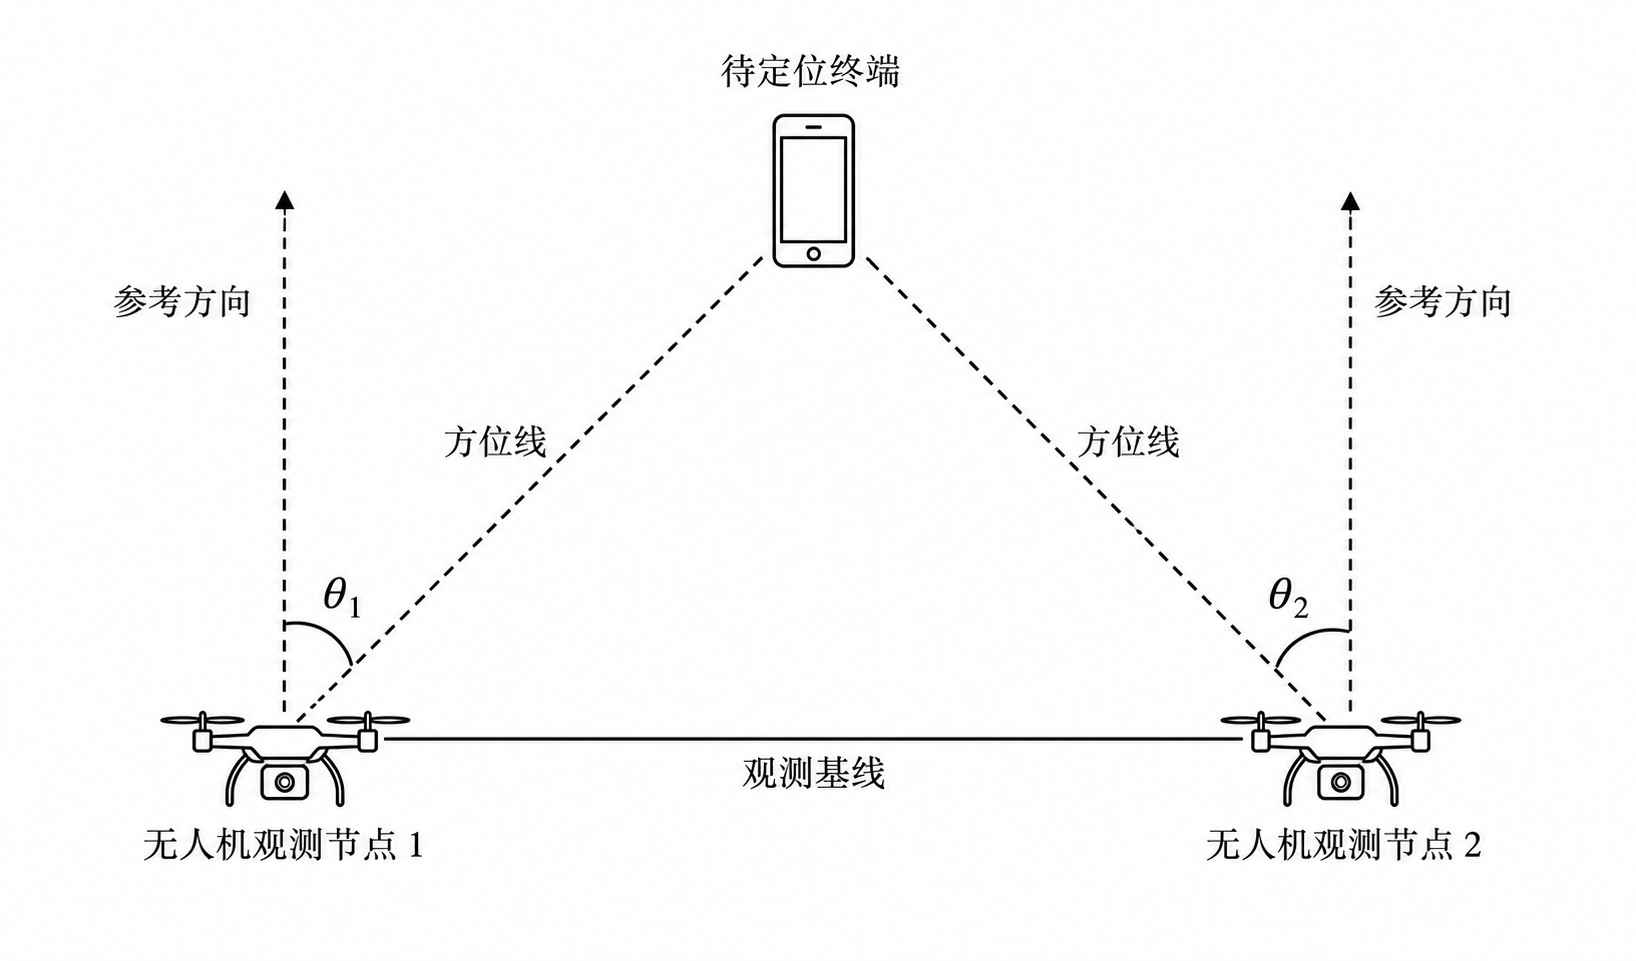
\includegraphics[width=0.78\textwidth]{figures/ch2/AOA.jpg}
    \caption{AOA 定位几何约束}
    \label{fig:ch2_aoa_localization}
\end{figure}

\subsection{TOA 定位}
\label{subsec:2_3_3}

TOA（Time of Arrival）定位方法通过测量信号从发射端传播到接收端的绝对到达时间实现对传播距离的估计。设第 $i$ 个接收机测得传播时延为 $t_i$，则距离满足 $\hat{d}_i=ct_i$。其几何约束为：
\begingroup
\setlength{\abovedisplayskip}{6pt}
\setlength{\belowdisplayskip}{6pt}
\setlength{\abovedisplayshortskip}{6pt}
\setlength{\belowdisplayshortskip}{6pt}
\begin{equation}
\sqrt{(x-x_i)^2+(y-y_i)^2}=ct_i,
\label{eq:2_19_toa_circle}
\end{equation}
\endgroup
这意味着每个 TOA 观测对应一条以接收机为圆心的等距圆。图~\ref{fig:ch2_toa_localization} 展示了 TOA 定位的测距几何关系。TOA 在理想条件下具有清晰的距离物理意义，且理论定位精度较高，但其前提是系统能够获得高精度绝对时间同步。对于本文所研究的非合作低轨卫星终端定位场景而言，目标发射时刻不可控，且复杂城市环境中的多径和非视距传播会进一步扰动时延测量结果，因此 TOA 更适合作为理论参照或基础观测模型，而难以直接作为本文的主定位路线\cite{Guvenc2009TOASurvey,Qin2025Timing}。

\begin{figure}[H]
    \centering
    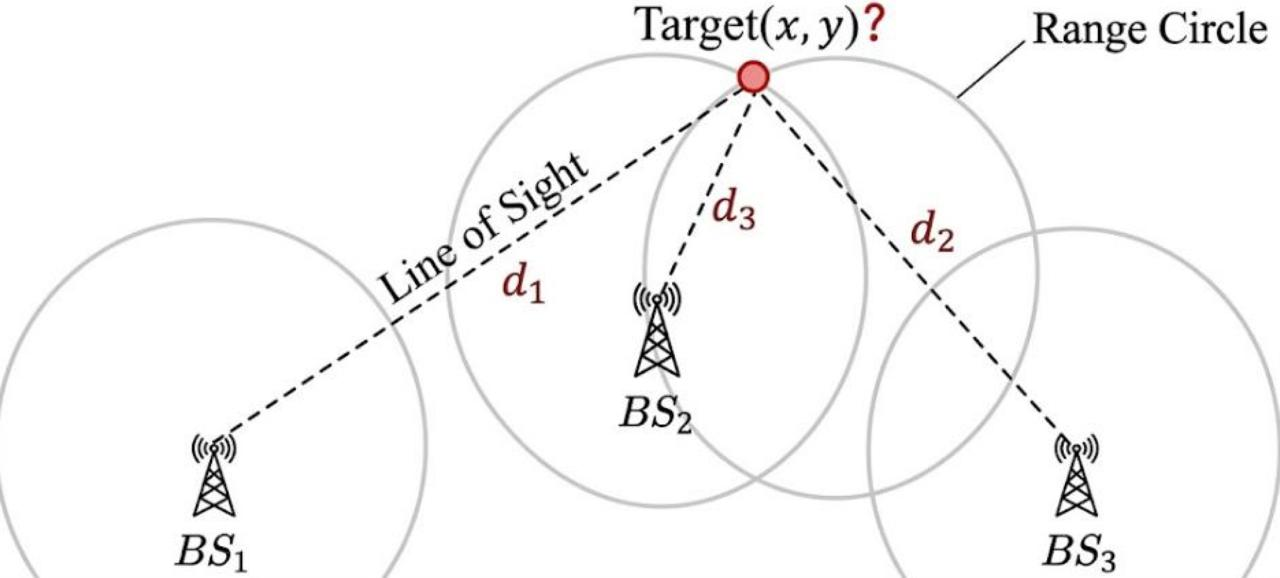
\includegraphics[width=0.78\textwidth]{figures/ch2/TOA.jpg}
    \caption{TOA 定位几何约束}
    \label{fig:ch2_toa_localization}
\end{figure}

\subsection{TDOA 定位}
\label{subsec:2_3_4}

TDOA（Time Difference of Arrival）定位方法通过不同接收机之间的到达时间差消除未知发射时刻的影响。设目标到第 $i$ 个接收机和参考接收机 1 的传播距离分别为 $d_i$ 和 $d_1$，则有：
\begingroup
\setlength{\abovedisplayskip}{6pt}
\setlength{\belowdisplayskip}{6pt}
\setlength{\abovedisplayshortskip}{6pt}
\setlength{\belowdisplayshortskip}{6pt}
\begin{equation}
\sqrt{(x-x_i)^2+(y-y_i)^2}-\sqrt{(x-x_1)^2+(y-y_1)^2}=c\Delta t_{i,1},
\label{eq:tdoa_hyperbola}
\end{equation}
\endgroup
式~\eqref{eq:tdoa_hyperbola} 对应一条双曲线，因此 TDOA 的定位本质是利用多条双曲线的交会确定目标位置。图~\ref{fig:ch2_tdoa_localization} 描绘了基于双曲线交会的 TDOA 定位原理。相较于 TOA，TDOA 不需要知道目标的绝对发射时刻，因此在非合作定位中具有更强的工程实用性。然而，TDOA 仍依赖多接收节点之间的严格时间同步以及较稳定的传播条件；在低成本无人机平台与复杂城市环境共同约束下，这类条件往往难以长期满足。因此，TDOA 在本文中更适合作为经典对比方法与理论分析基础，而不是后续方法设计的主要技术路线\cite{Chan1994Hyperbolic,Guvenc2009TOASurvey,Torrieri1984PassiveLocation}。

\begin{figure}[H]
    \centering
    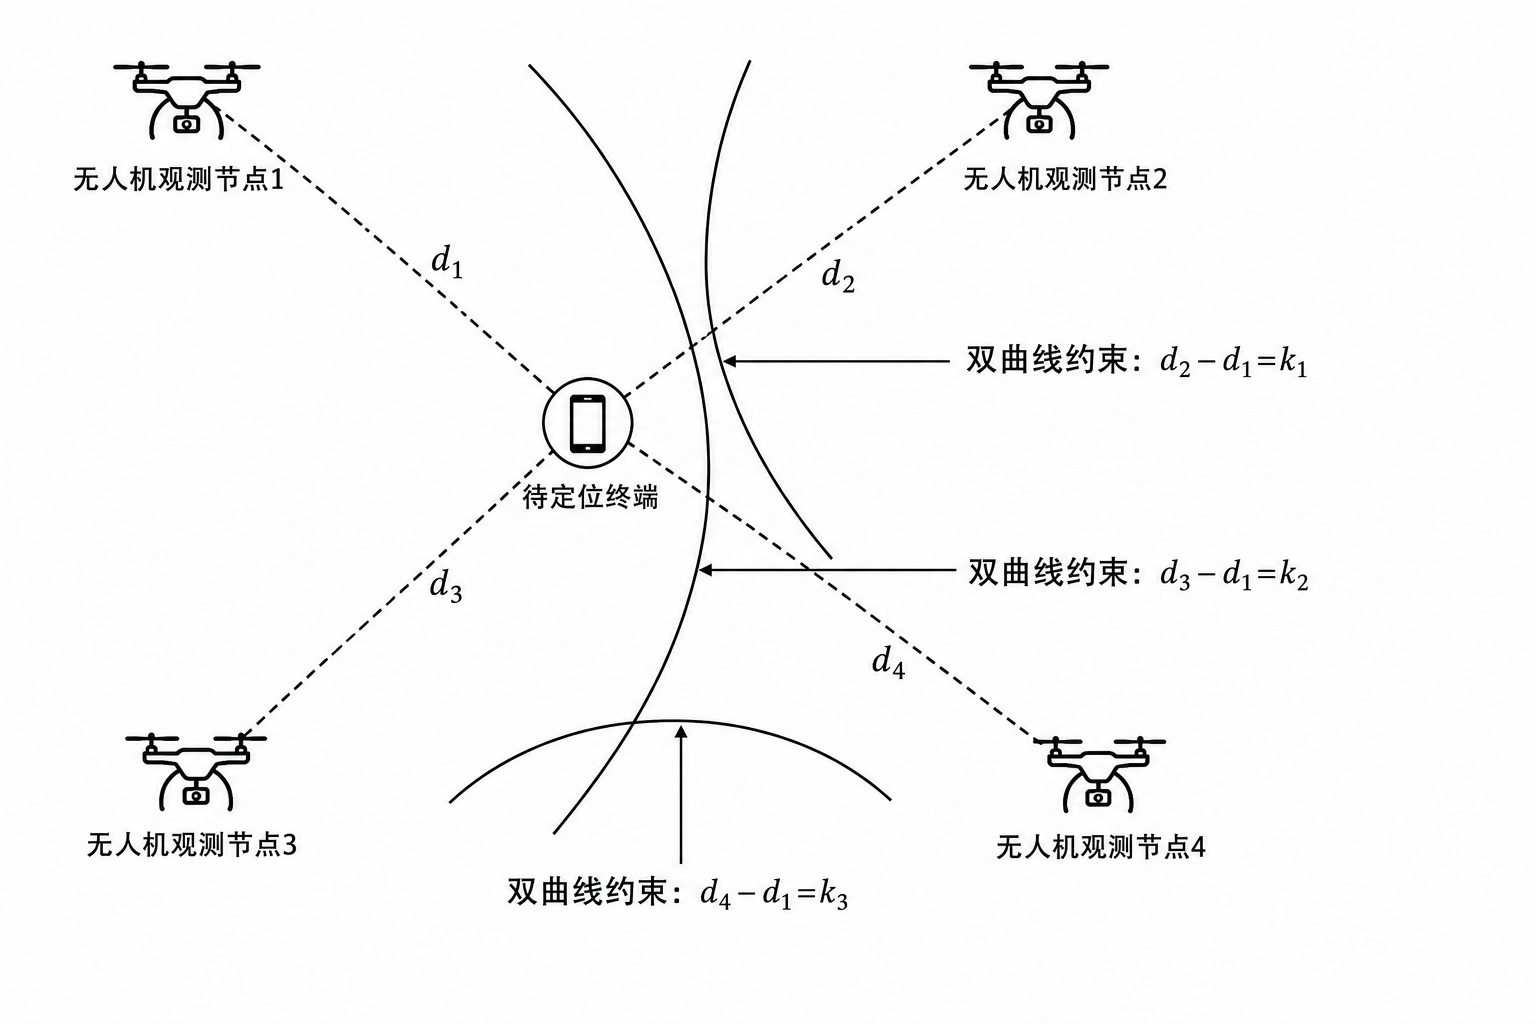
\includegraphics[width=0.78\textwidth]{figures/ch2/TDOA.jpg}
    \caption{TDOA 定位几何约束}
    \label{fig:ch2_tdoa_localization}
\end{figure}

\subsection{PDR 定位}
\label{subsec:2_3_5}

位置递推（Pedestrian Dead Reckoning, PDR）是一种利用先验运动学模型，通过积分或离散累加前一时刻的位置来推算当前位置的手段。在离散时间二维空间中，PDR 定位模型的标准状态更新公式可表示为：
\begin{equation}
\begin{bmatrix} x_k \\ y_k \end{bmatrix} = \begin{bmatrix} x_{k-1} \\ y_{k-1} \end{bmatrix} + \Delta d_k \begin{bmatrix} \cos \theta_k \\ \sin \theta_k \end{bmatrix} + \mathbf{w}_k,
\label{eq:2_21_pdr_update}
\end{equation}
其中，$(x_k, y_k)^T$ 表示目标在 $k$ 时刻的二维坐标，$\Delta d_k$ 为步长，$\theta_k$ 为运动航向角，$\mathbf{w}_k$ 为过程噪声。图~\ref{fig:ch2_pdr_localization} 给出了 PDR 运动递推的基本逻辑示意。PDR 方法的优势在于其完全自主，不受城市峡谷中多径和信号衰落的影响，但其缺陷在于误差会随时间累积产生偏移（Drift Error）。

\begin{figure}[H]
    \centering
    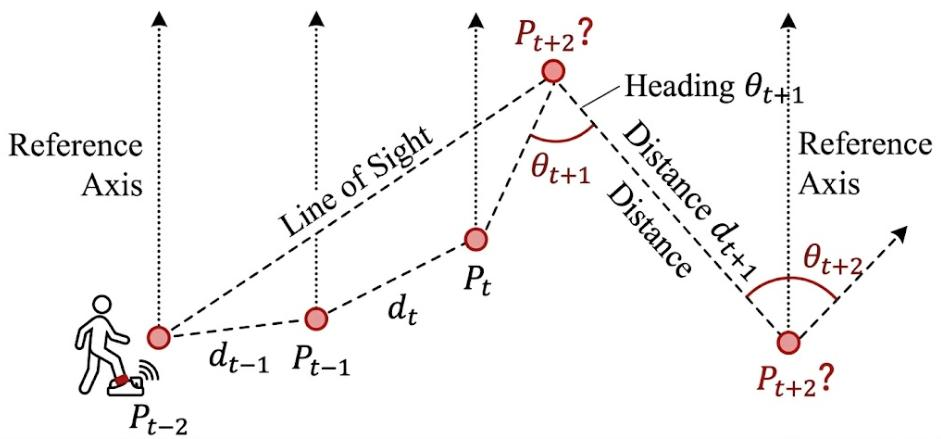
\includegraphics[width=0.78\textwidth]{figures/ch2/PDR.jpg}
    \caption{PDR 定位运动递推过程}
    \label{fig:ch2_pdr_localization}
\end{figure}
\section{面向定位的监督学习与知识迁移基础}
\label{sec:2_4}

前文已对低轨卫星信号模型以及 RSSI、AOA、TOA、TDOA 和 PDR 等经典定位方法进行了分析。在低成本无人机平台与复杂传播环境的共同约束下，定位系统进一步面临两类关键问题：对于单目标连续定位，观测可靠性和环境状态随时间变化，需要依据当前传播特征和多源定位结果之间的相互关系动态调整融合权重；对于多无人机协同定位，节点掉点和观测残缺会削弱空间判别能力，需要将完整观测条件下获得的定位知识迁移至不完整观测场景。

基于上述考虑，本节介绍与后续方法直接相关的两类理论基础：面向单目标融合权重预测的监督学习基础，以及面向残缺观测鲁棒定位的知识蒸馏基础。其中，前者主要服务于第三章中的单目标自适应融合定位建模，后者主要服务于第四章中的多目标协同鲁棒定位建模。

\subsection{XGBoost 梯度提升回归基础}
\label{subsec:2_4_1}

极端梯度提升（Extreme Gradient Boosting, XGBoost）是一类基于梯度提升决策树的集成学习算法\cite{Chen2016XGBoost}。其基本思想并非由单棵决策树一次性完成全部拟合，而是通过多棵回归树的加法集成，在每一轮训练中让新树拟合当前残差，从而逐步逼近目标值。对于第三章中的融合权重预测任务，输入为由 RMS 时延扩展、RSSI 统计量及多源一致性距离等构成的低维特征向量 $\mathbf{t}_k\in\mathbb{R}^{6}$，输出为离线反解得到的最优融合权重标签 $q_{k,i}^{\ast}$，因此 XGBoost 在本文中执行的是连续值回归，而非分类任务。

设第 $i$ 个权重分量（$i=1,2,3$ 分别对应 AoA、PDR 和 RSSI）对应的训练样本为
\begin{equation}
\mathcal{D}_i
=
\left\{
\left(\mathbf{t}_k,\,q_{k,i}^{\ast}\right)
\right\}_{k=1}^{N},
\label{eq:2_25_xgb_dataset}
\end{equation}
则可将权重预测建模为从特征空间到标量权重的映射 $f_i:\mathbb{R}^{6}\rightarrow\mathbb{R}$。第 $i$ 个 XGBoost 回归器由 $M$ 棵 CART 回归树组成，其加法模型可写为
\begin{equation}
\tilde{q}_{k,i}
=
\hat{q}_{k,i}^{(0)}
+
\eta
\sum_{m=1}^{M}
f_{i,m}(\mathbf{t}_k),
\label{eq:2_26_xgb_additive}
\end{equation}
其中，$\hat{q}_{k,i}^{(0)}$ 为初始预测值，$\eta$ 为学习率，$f_{i,m}(\cdot)$ 表示第 $m$ 棵回归树。每棵树依据特征阈值划分样本空间，并在叶节点输出连续数值，由此实现对 $\mathbf{t}_k$ 与 $q_{k,i}^{\ast}$ 之间非线性关系的逼近。

XGBoost 在每一轮新增树时，并不仅追求训练误差下降，还通过正则项约束模型复杂度。以第 $i$ 个权重分量为例，其训练目标可表示为
\begin{equation}
\mathcal{L}_i
=
\sum_{k=1}^{N}
l\left(q_{k,i}^{\ast},\,\tilde{q}_{k,i}\right)
+
\sum_{m=1}^{M}
\Omega(f_{i,m}),
\label{eq:2_27_xgb_objective}
\end{equation}
其中，$l(\cdot)$ 为回归损失函数，第三章采用平方误差损失；$\Omega(f)$ 为树复杂度正则项，常写为
\begin{equation}
\Omega(f)
=
\gamma T_f
+
\frac{1}{2}
\lambda
\sum_{j=1}^{T_f}
w_j^2,
\label{eq:2_28_xgb_regularization}
\end{equation}
其中，$T_f$ 为叶节点数量，$w_j$ 为第 $j$ 个叶节点输出，$\gamma$ 与 $\lambda$ 分别约束树结构与叶节点输出幅度。由于 AoA、PDR 和 RSSI 三路权重需同时预测，第三章将任务分解为三个独立的标量回归器分别训练；预测完成后对权重进行仿射归一化，以满足融合模型中的权重和约束。式~\eqref{eq:2_26_xgb_additive}--式~\eqref{eq:2_28_xgb_regularization} 构成第三章 XGBoost 权重回归模型的理论依据，具体特征构造、标签反解与在线推理流程将在第三章中展开。

\subsection{知识蒸馏基础}
\label{subsec:2_4_2}

除面向单目标融合权重学习的监督回归方法外，本文第四章还涉及另一类重要的学习机制，即知识蒸馏（Knowledge Distillation）。在多无人机协同定位场景中，随机掉点、节点失效和观测残缺会导致输入信息不完整，从而削弱模型对目标空间位置的判别能力。知识蒸馏的基本思想是利用性能更强、输入信息更完整或训练更充分的教师模型，将其学习到的定位判别知识迁移给学生模型，使后者在观测残缺条件下仍能够逼近教师模型的性能。

在本文场景下，教师模型通常对应完整观测条件下的定位网络，学生模型则对应掉点或残缺观测条件下的定位网络。若分别记完整观测输入和残缺观测输入为 $\mathbf{X}^{\mathrm{full}}$ 与 $\mathbf{X}^{\mathrm{drop}}$，则二者的输出 logits 可表示为
\begin{equation}
\mathbf{z}^{T}=f_T(\mathbf{X}^{\mathrm{full}}),
\qquad
\mathbf{z}^{S}=f_S(\mathbf{X}^{\mathrm{drop}}),
\label{eq:2_32_kd_input}
\end{equation}
其中，$f_T(\cdot)$ 和 $f_S(\cdot)$ 分别表示教师网络和学生网络。在教师—学生框架下，设教师网络输出 logits 向量为 $\mathbf{z}^{T}$，学生网络输出 logits 向量为 $\mathbf{z}^{S}$，则在温度系数 $T_d$ 作用下，教师网络的软标签分布可表示为
\begin{equation}
q^{T}_{m}
=
\frac{\exp(z^{T}_{m}/T_d)}
{\sum_{n}\exp(z^{T}_{n}/T_d)},
\label{eq:2_32_teacher_soft}
\end{equation}
学生网络对应的软化输出为
\begin{equation}
q^{S}_{m}
=
\frac{\exp(z^{S}_{m}/T_d)}
{\sum_{n}\exp(z^{S}_{n}/T_d)}.
\label{eq:2_33_student_soft}
\end{equation}
其中，$m$ 表示第 $m$ 个空间栅格或候选定位区域索引。相比于 one-hot 硬标签，软标签分布包含了不同空间位置之间更细粒度的相对相似性信息，因此能够为学生网络提供更丰富的监督信号\cite{Hinton2015KD}。对于基于空间栅格的定位判别任务，学生网络的最终位置输出可进一步写为
\begin{equation}
\hat{m}
=
\arg\max_m q_m^S,
\qquad
\hat{\mathbf{p}}
=
\mathbf{c}_{\hat{m}},
\label{eq:2_34_kd_position}
\end{equation}
其中，$\mathbf{c}_{\hat{m}}$ 表示预测栅格中心对应的位置坐标。该式表明，知识蒸馏所迁移的并非一般分类知识，而是面向空间栅格定位任务的区域判别能力；在本文第四章中，这种能力进一步体现为完整协同观测条件下的空间结构知识向残缺观测条件下定位模型的迁移。

图~\ref{fig:ch2_distillation_framework} 展示了知识蒸馏中典型的教师—学生学习架构。通过该机制，学生网络能够在缺失部分节点观测的条件下，通过学习教师模型的判别特征维持定位性能的稳健性。

\begin{figure}[htbp]
    \centering
    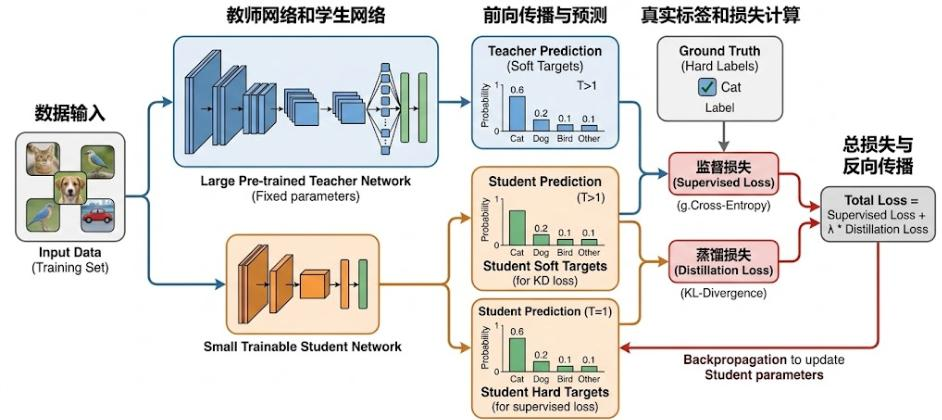
\includegraphics[width=0.82\textwidth]{figures/ch2/KD.jpg}
    \caption{知识蒸馏教师—学生学习机制}
    \label{fig:ch2_distillation_framework}
\end{figure}

综上，知识蒸馏通过引入教师模型的软标签监督，为观测不完整条件下的学生定位模型提供了更强的空间判别引导能力。这一机制在本文中并非主要用于一般意义上的模型压缩，而是服务于多无人机掉点条件下协同定位能力的知识迁移，从而为第四章面向残缺观测场景的鲁棒定位方法提供直接理论基础。

\section{定位性能评估}
\label{sec:2_5}

在完成经典定位模型以及面向定位的监督学习与知识迁移基础介绍之后，还需要进一步给出本文后续实验分析中采用的性能评估方式。对于定位问题而言，方法优劣最终需要通过定量指标进行衡量，而这些指标既应反映整体精度，也应能够刻画极端误差和理论性能上限。基于这一考虑，本文从定位误差评价指标和克拉美罗下界两个角度，对定位性能评估基础进行说明。

\subsection{定位误差评价指标}
\label{subsec:2_5_1}

定位误差是衡量定位系统性能最直接的指标。设目标真实位置为
\begin{equation}
\mathbf{p}^{\mathrm{gt}}
=
[x^{\mathrm{gt}},y^{\mathrm{gt}}]^T,
\label{eq:2_36_gt_position}
\end{equation}
定位算法输出的位置估计为
\begin{equation}
\hat{\mathbf{p}}
=
[\hat{x},\hat{y}]^T,
\label{eq:2_37_est_position}
\end{equation}
则单次定位误差可定义为二者之间的欧氏距离
\begin{equation}
e
=
\left\|
\hat{\mathbf{p}}-\mathbf{p}^{\mathrm{gt}}
\right\|_2
=
\sqrt{
(\hat{x}-x^{\mathrm{gt}})^2
+
(\hat{y}-y^{\mathrm{gt}})^2
}.
\label{eq:2_38_single_error}
\end{equation}
若共有 $N$ 个测试样本，则平均定位误差（Mean Localization Error）可表示为
\begin{equation}
\mathrm{Mean\ Localization\ Error}
=
\frac{1}{N}\sum_{i=1}^{N} e_i,
\label{eq:2_39_mean_error}
\end{equation}
均方根误差（RMSE）可表示为
\begin{equation}
\mathrm{RMSE}
=
\sqrt{
\frac{1}{N}\sum_{i=1}^{N} e_i^2
},
\label{eq:2_40_rmse}
\end{equation}
其中，$e_i$ 表示第 $i$ 个样本的定位误差。平均定位误差用于反映整体平均偏差水平，RMSE 则对较大误差更为敏感，因此更适合作为总体精度的综合衡量指标。

除均值类指标外，尾部误差指标同样具有重要意义。对于连续定位或复杂环境定位任务而言，偶发性的大误差往往会直接导致轨迹推算跳变、目标误判或系统失稳。因此，本文后续还将使用百分位误差，如 $90\%$ 分位误差或 $95\%$ 分位误差，对误差分布尾部进行刻画。若记误差样本按从小到大排序后的 $p\%$ 分位值为 $e_{p}$，则其含义为：有 $p\%$ 的测试样本定位误差不超过该值。与均值指标相比，百分位误差更能反映系统在极端场景下的稳定性与工程可用性。

此外，在后续多目标定位实验中，还将进一步采用误差累计分布函数（CDF）对整体误差分布进行描述。CDF 曲线的横轴表示误差阈值，纵轴表示误差不超过该阈值的样本累计比例。该图形化指标能够较直观地比较不同方法在整体误差分布上的优劣，尤其适合展示蒸馏增强模型与未增强模型之间的差异。

综上，本文后续实验中采用的定位误差评价指标将主要包括平均定位误差、RMSE、百分位误差以及误差 CDF 曲线等形式。它们分别对应整体平均性能、较大误差敏感性、尾部鲁棒性和误差分布形态，从不同角度共同支撑定位性能分析。

\subsection{克拉美罗下界分析基础}
\label{subsec:2_5_2}

除实验统计指标外，克拉美罗下界（Cramér--Rao Lower Bound, CRLB）也是分析定位系统理论性能的重要工具。其基本作用在于：在给定观测模型与噪声统计条件下，给出无偏估计器协方差所能达到的理论下界，从而反映系统在理想条件下的最优可达性能\cite{Torrieri1984PassiveLocation,Wymeersch2009CooperativeLocalization}。

对于一般定位问题，可将观测模型统一写为
\begin{equation}
\mathbf{z}
=
\mathbf{h}(\mathbf{p})
+
\mathbf{n},
\label{eq:2_41_general_obs}
\end{equation}
其中，$\mathbf{p}=[x,y]^T$ 为待估位置参数，$\mathbf{z}$ 为观测向量，$\mathbf{h}(\mathbf{p})$ 为位置到观测空间的映射函数，$\mathbf{n}$ 为观测噪声。若噪声协方差矩阵为 $\mathbf{R}$，则 Fisher 信息矩阵可表示为
\begin{equation}
\mathbf{J}(\mathbf{p})
=
\left(
\frac{\partial \mathbf{h}}{\partial \mathbf{p}}
\right)^T
\mathbf{R}^{-1}
\left(
\frac{\partial \mathbf{h}}{\partial \mathbf{p}}
\right),
\label{eq:2_42_fim}
\end{equation}
其中，$\frac{\partial \mathbf{h}}{\partial \mathbf{p}}$ 表示观测函数对位置参数的雅可比矩阵。

在无偏估计条件下，位置估计协方差满足
\begin{equation}
\mathrm{Cov}(\hat{\mathbf{p}})
\succeq
\mathbf{J}^{-1}(\mathbf{p}),
\label{eq:2_43_crlb_cov}
\end{equation}
即任何无偏估计器的误差协方差都不可能优于 Fisher 信息矩阵逆所给出的下界。进一步地，对于二维定位问题，其均方根误差下界可写为
\begin{equation}
\mathrm{RMSE}
\ge
\sqrt{
\mathrm{tr}
\left(
\mathbf{J}^{-1}(\mathbf{p})
\right)
}.
\label{eq:2_44_crlb_rmse}
\end{equation}
CRLB 的意义在于，它不依赖于具体求解算法，而仅由观测模型和噪声统计决定。因此，可利用 CRLB 对不同观测量组合在理想条件下的理论可达精度进行比较。例如，对于 RSSI、AOA、TOA 和 TDOA 等经典方法，若其观测模型和噪声特性已知，则均可通过式~\eqref{eq:2_42_fim}--式~\eqref{eq:2_44_crlb_rmse} 计算理论误差下界\cite{Torrieri1984PassiveLocation,Wymeersch2009CooperativeLocalization}。

需要指出的是，复杂城市环境中的实际定位误差通常会高于理想 CRLB。其原因在于，CRLB 假设观测模型准确且噪声统计可知，而现实环境中广泛存在多径传播、非视距偏差、模型失配和观测异常等问题，这些因素都会使实际误差偏离理想下界。然而，即便如此，CRLB 仍然是分析定位理论性能上限的重要参照。对于本文而言，它的价值更多体现在理论层面：一方面说明不同观测模型的潜在精度差异，另一方面为后续实验结果分析提供理想性能对照。

综上，定位误差评价指标与克拉美罗下界共同构成了本文后续章节的性能分析基础。前者用于从实验层面定量评估定位方法的实际效果，后者则用于从理论层面衡量观测模型的可达性能边界。二者结合后，可较完整地支撑后续第三章与第四章中的实验结果分析与方法比较。

\section{本章小结}
\label{sec:2_6}

本章围绕低成本无人机平台下的非合作终端定位问题，系统梳理了后续研究所需的系统模型与理论基础。首先，结合手机直连卫星场景下的终端排查任务特点，给出了低成本无人机机动观测场景下的系统任务描述与总体架构，明确了本文所研究问题属于复杂城市环境中的非合作式无源定位问题。其次，围绕目标外部观测信号模型，对复杂城市环境中的多径效应、时延扩展和信号衰落机制进行了分析，为后续物理特征提取与定位方法设计提供了基础。

在此基础上，本章进一步总结了 RSSI、AOA、TOA、TDOA 和 PDR 等经典定位方法模型，分析了不同观测量所对应的几何约束关系及其在复杂城市环境中的适用边界。相关分析表明，在低成本无人机平台与复杂传播环境的双重约束下，单一经典定位观测量往往难以同时兼顾高精度、强鲁棒和低复杂度，这为后续引入多源融合、监督权重学习与知识蒸馏等方法提供了问题背景。

最后，本章从学习方法基础与性能评估基础两个方面，为后续章节展开做了铺垫。监督权重学习与 XGBoost 梯度提升回归基础，为第三章中基于一致性增强监督权重学习的单目标自适应融合定位方法提供了理论支撑；知识蒸馏基础，则为第四章中面向多无人机掉点场景的鲁棒定位方法奠定了理论基础。同时，平均定位误差、RMSE、百分位误差以及克拉美罗下界等性能评估指标，也为后续实验分析提供了统一评价依据。

进一步地，本章所建立的理论基础并不是彼此孤立的若干模型堆叠，而是围绕复杂城市环境下非合作低轨卫星终端定位这一核心任务逐层展开：系统任务描述给出了应用背景，信号模型刻画了传播约束，经典定位模型揭示了单一观测量的局限，而监督学习与知识迁移基础则给出了后续方法设计的求解路径。由此，第二章在全文中承担了由任务问题向方法建模过渡的桥梁作用。

综上，本章完成了从任务场景、信号模型、经典定位模型到学习方法基础的整体铺垫，为后续第三章单目标连续定位方法和第四章多目标并发定位方法的研究奠定了统一的理论基础。
